\documentclass[10pt,aspectratio=169]{beamer}
\usetheme{default}
\setbeamercovered{invisible}
\setbeamertemplate{navigation symbols}{}
\setbeamertemplate{footline}{
    \flushright{\hfill \insertframenumber{}/\inserttotalframenumber}
}

\usepackage{listings}

% User-defined colors.
\definecolor{DarkGreen}{rgb}{0, .5, 0}
\definecolor{DarkBlue}{rgb}{0, 0, .5}
\definecolor{DarkRed}{rgb}{.5, 0, 0}
\definecolor{LightGray}{rgb}{.95, .95, .95}
\definecolor{White}{rgb}{1.0,1.0,1.0}
\definecolor{darkblue}{rgb}{0,0,0.9}
\definecolor{darkred}{rgb}{0.8,0,0}
\definecolor{darkgreen}{rgb}{0.0,0.85,0}

% Settings for listing class.
\lstset{
  language=C++,                        % The default language
  basicstyle=\small\ttfamily,          % The basic style
  backgroundcolor=\color{White},       % Set listing background
  keywordstyle=\color{DarkBlue}\bfseries, % Set keyword style
  commentstyle=\color{DarkGreen}\itshape, % Set comment style
  stringstyle=\color{DarkRed}, % Set string constant style
  extendedchars=true % Allow extended characters
  breaklines=true,
  basewidth={0.5em,0.4em},
  fontadjust=true,
  linewidth=\textwidth,
  breakatwhitespace=true,
  showstringspaces=false,
  lineskip=0ex, %  frame=single
}

\begin{document}
    \title{Optimization and profiling}
    \author{Matteo Caldana}
    \date{04/05/2023}

\begin{frame}[plain, noframenumbering]
    \maketitle
\end{frame}

\begin{frame}{CPU vs. RAM}
    \begin{figure}
        \centering
        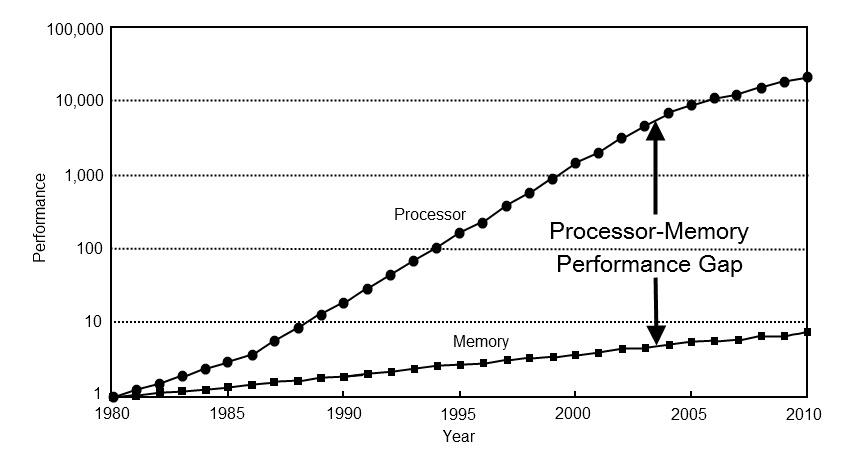
\includegraphics[width=0.9\textwidth]{images/cpu_memory_performance_gap.png}
        \caption{\textit{Computer Architecture: A Quantitative Approach by John L. Hennessy, David A. Patterson, Andrea C. Arpaci-Dusseau}}
    \end{figure}
\end{frame}

\begin{frame}{Memory layout}
    \begin{figure}
        \centering
        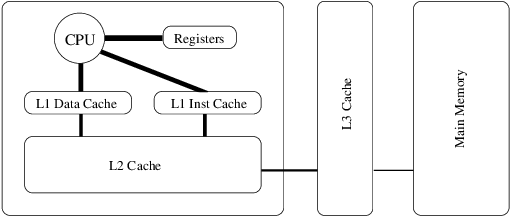
\includegraphics[width=\textwidth]{images/memory_layout.png}
        \caption{Typical memory layout of a computer.}
    \end{figure}
\end{frame}

\begin{frame}{Cache miss}
    \begin{figure}
        \centering
        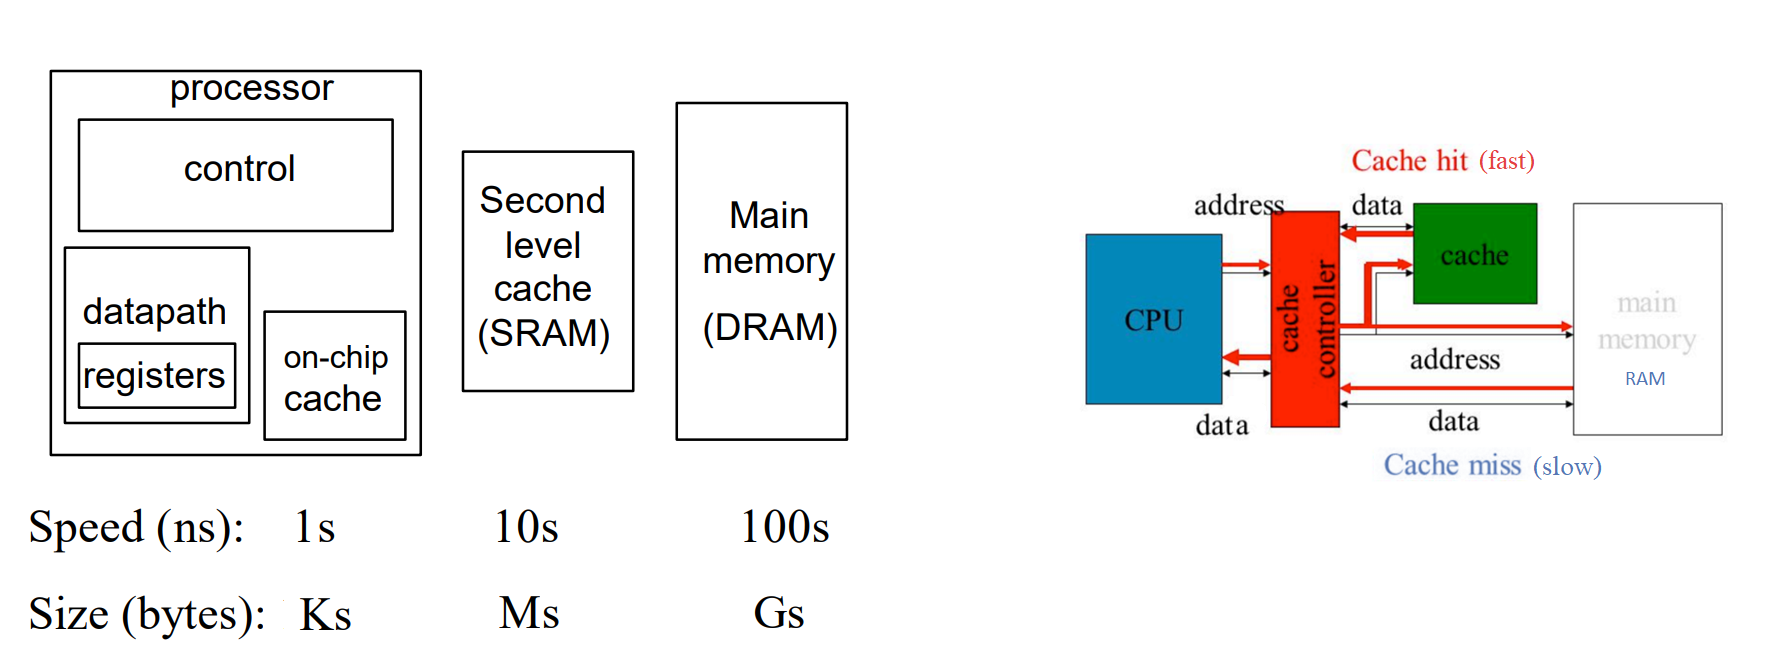
\includegraphics[width=\textwidth]{images/cache.png}
        \caption{Typical access times to memory. \footnote{See also: \url{https://en.wikipedia.org/wiki/Cache_performance_measurement_and_metric}, \url{https://en.wikipedia.org/wiki/Cache_hierarchy}}}
    \end{figure}
\end{frame}

\begin{frame}{Exercise 1 - How memory access affects performance}
    This exercise is inspired by \href{https://bitbashing.io/memory-performance.html}{\textcolor{DarkBlue}{this post}}.
    \vfill
    The source file \texttt{01-memory-access/01-base.cpp} implements a very simple algorithm, where a \texttt{std::vector} of size equal to an integer multiple of the cache memory is filled with random numbers and applied some simple mathematical operation (function \texttt{compute()}) for a specified amount of iterations.
    \vfill
    Compare the performance of the following three ways of accessing elements in the vector:
    \begin{enumerate}
        \item sequential value access;
        \item sequential pointer access;
        \item random pointer access.
    \end{enumerate}
\end{frame}

\begin{frame}{Exercise 2 - Optimization techniques\footnote{See also: \url{https://github.com/ArtemKovera/code-optimization-techniques}}}
    \begin{enumerate}
        \item Implement a function that allocates a \texttt{std::vector} and, taking an index as an input, simply returns the corresponding value. Compare the performance with respect to declaring the vector \texttt{static}.
        \item Implement a function that multiplies all elements in a \texttt{std::vector} by looping over all its elements and returns the result. Compare the performance with respect to rewriting the loop using unrolling. That is, at each iteration multiply together five elements of the vector \footnote{See also: \url{https://en.wikipedia.org/wiki/Loop_unrolling}}.
        \item Optimize the memory occupation of an object of class \texttt{Class1} by properly aligning/padding the data structure.
    \end{enumerate}
\end{frame}

\begin{frame}[fragile]{Data structure alignment\footnote{See also: \url{https://www.geeksforgeeks.org/data-structure-alignment/}}}
    \begin{lstlisting}
class MyClass
{
  char a;      // 1 byte.
  short int b; // 2 bytes.
  int c;       // 4 bytes.
  char d;      // 1 bytes.
}
    \end{lstlisting}
    \begin{figure}
        \centering
        \only<1>{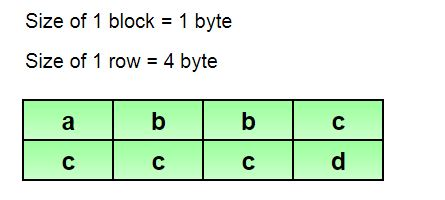
\includegraphics[width=0.45\textwidth]{images/padding_pre.jpg}}
        \only<2>{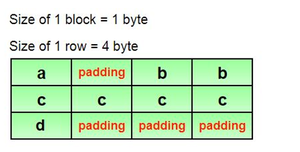
\includegraphics[width=0.45\textwidth]{images/padding_post.png}}
        \caption{How data is \alt<1>{\textbf{not}}{actually} stored.}
    \end{figure}
\end{frame}


\begin{frame}{Exercise 3 - Operating with matrices}
Starting from the provided implementation of the class for dense matrices (and column vectors represented as 1-column matrices) based on \lstinline{std::vector}, implement the following methods:
\begin{itemize}
\item \lstinline{transpose()}: $A = A^{T}$.
\item \lstinline{operator*}: matrix-matrix and matrix-vector multiplication.
\end{itemize}
\end{frame}

\begin{frame}{Exercise 3 - What you need to know}
\begin{itemize}
\item The implemented matrix class is organized as
      \textbf{column-major}, \textit{i.e.}
      $A(i, j) = $ \lstinline{data[i + j * n_rows()]},
      conversion from 1D to 2D indexing is performed by the utility
      method \lstinline{sub2ind}.\\[3mm]
\item Access to elements is implemented both in \texttt{const} and non-\texttt{const} versions, by overloading \lstinline{operator()} and the \texttt{value} method. \\[3mm]
\item Data is private, \textit{getter methods} expose what is needed to the user, both \texttt{const} and non-\texttt{const} versions are provided. \\[3mm]
\item Naive implementation of matrix-matrix multiplication is slow because it has low \textit{data locality}, simply transposing the left matrix factor improves performance significantly\footnote{See also: \textit{M. Kowarschik, C. Weiß. (2002). Lecture Notes in Computer Science. 213-232. DOI: 10.1007/3-540-36574-5\_10} for further details.}.\\[3mm]
\end{itemize}
\end{frame}

\begin{frame}{Matrix-matrix multiplication: access patterns}
    \begin{figure}
        \centering
        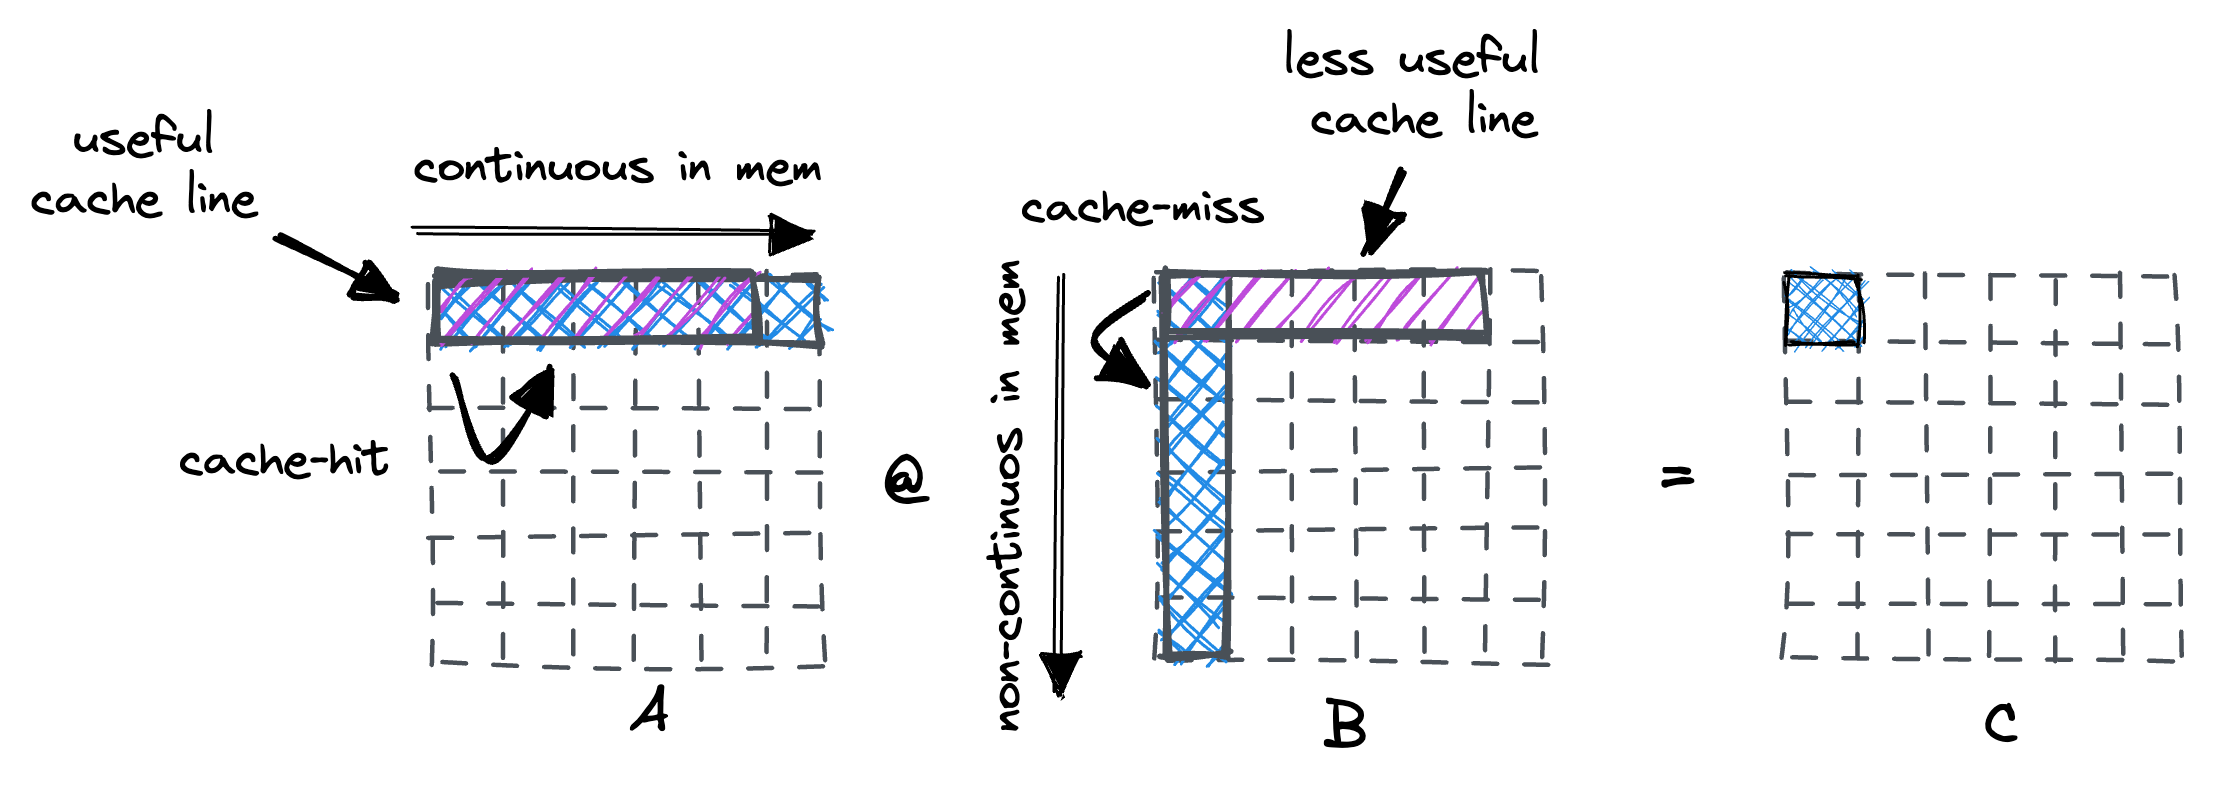
\includegraphics[width=\textwidth]{images/cache-unaware-dot-product.png}
        \caption{Access patterns for a \textbf{row-major} data structure, assuming that the cache can store 5 elements at once. If elements are accessed in column-wise order (blue pattern in matrix B) then the loop is \textbf{not} cache-friendly: at the second iterations the purple elements, that are already in the cache since their memory location is contiguous to the first one, are discarded: thus new entries must be re-cached (very expensive!). Analogous considerations hold for \textbf{column-major} data structures. Credits to: \url{https://siboehm.com/articles/22/Fast-MMM-on-CPU}}
    \end{figure}
\end{frame}

\begin{frame}{Matrix-matrix multiplication: cache aware}
    \begin{figure}
        \centering
        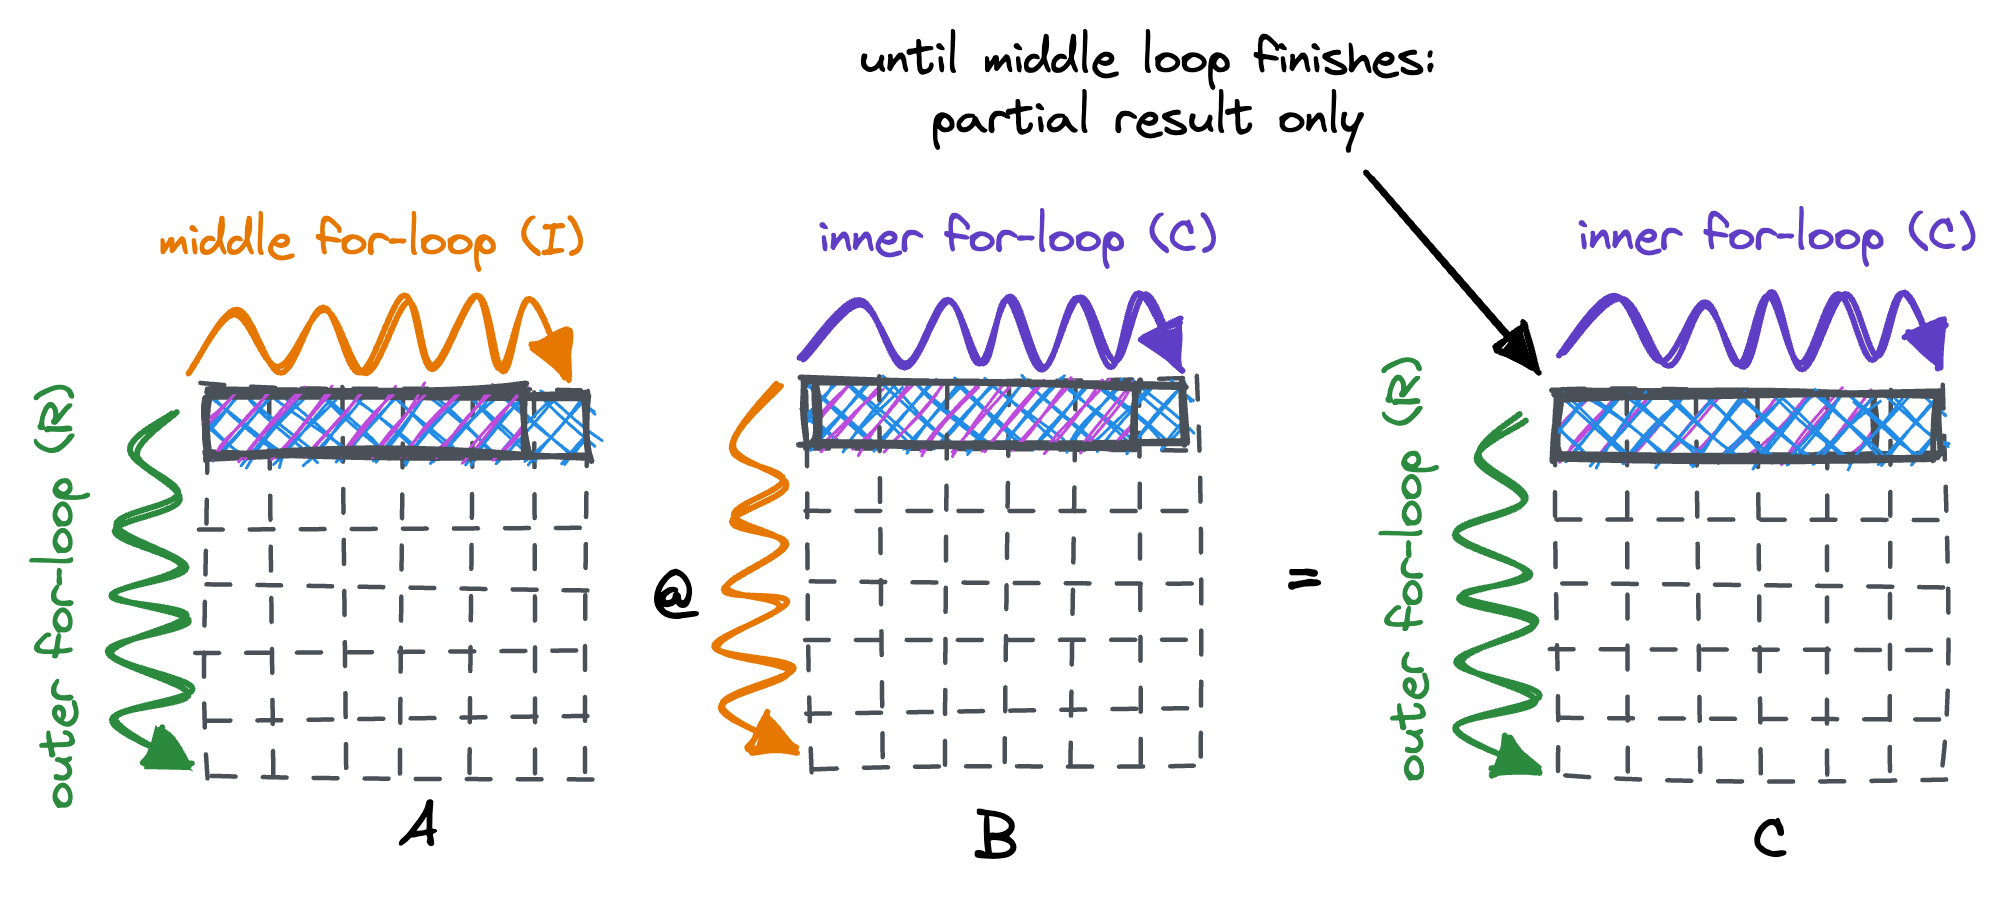
\includegraphics[width=\textwidth]{images/cache-aware-dot-prod-reorder-loops.png}
        \caption{By switching the two most inner for loops we have a cache-aware algorithm. Credits to: \url{https://siboehm.com/articles/22/Fast-MMM-on-CPU}}
    \end{figure}
\end{frame}

\begin{frame}{Matrix-matrix multiplication: loop tiling}
    \begin{figure}
        \centering
        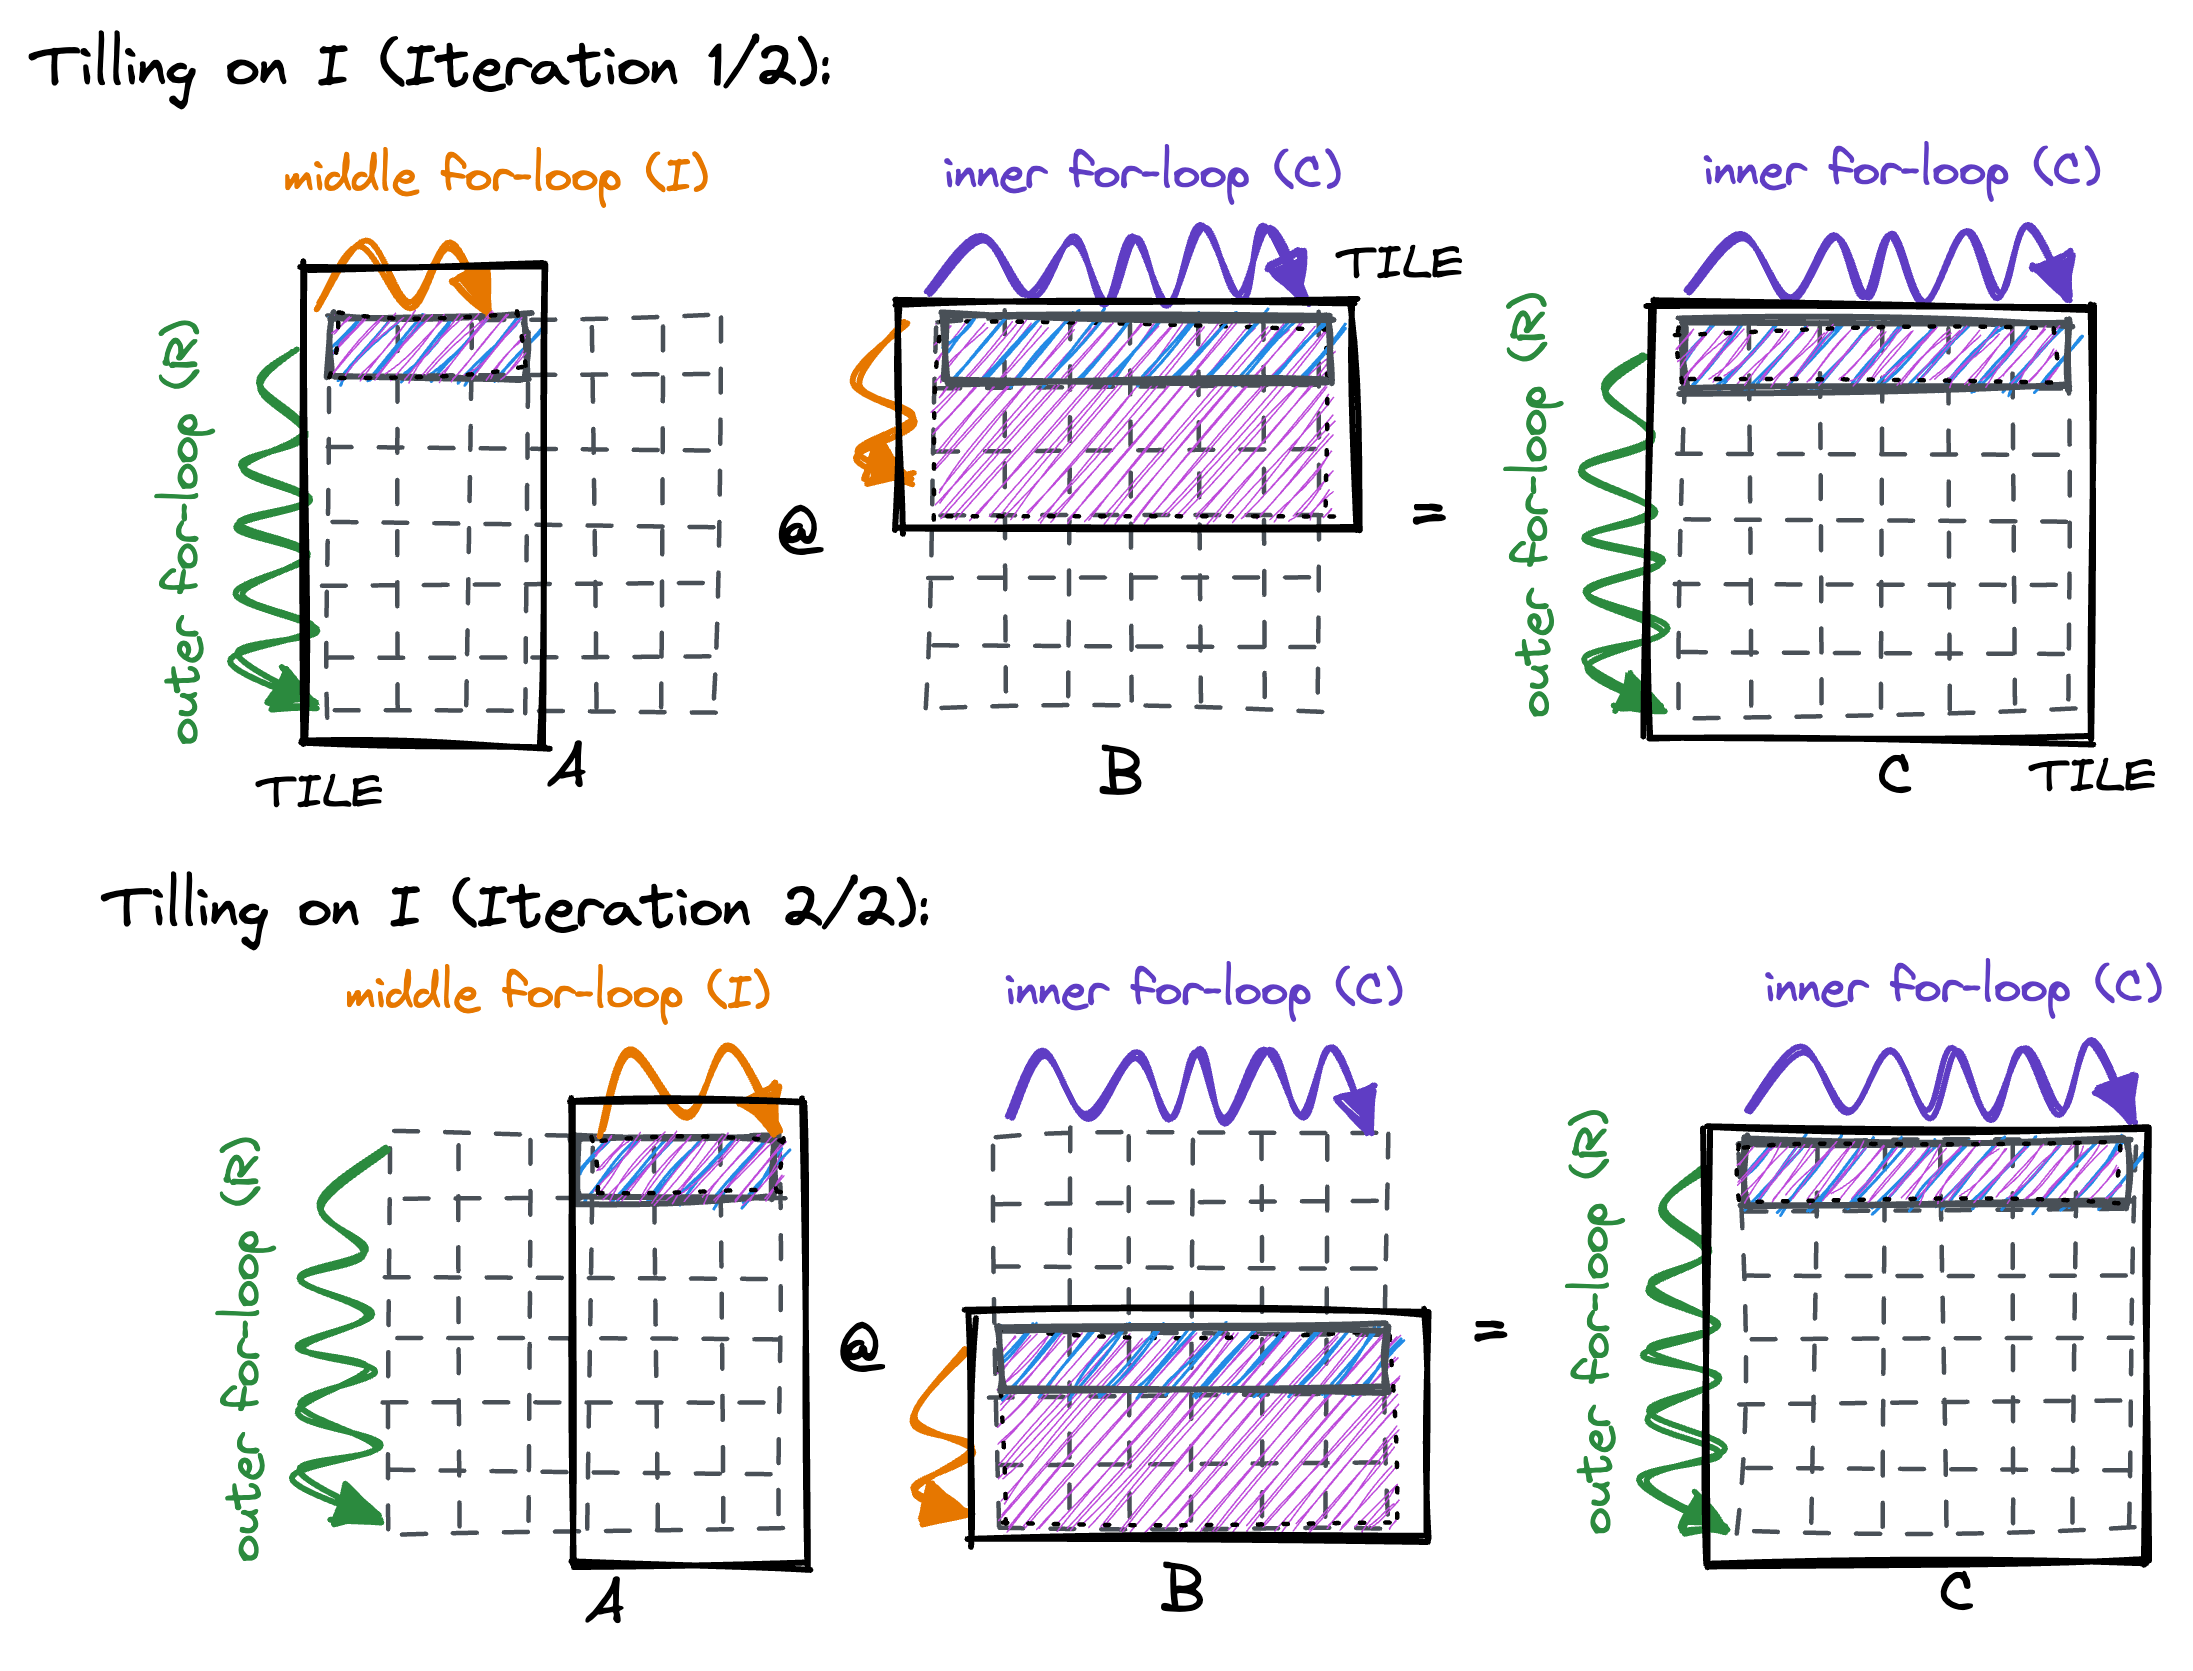
\includegraphics[width=0.65\textwidth]{images/Tiling_on_inner.png}
        \caption{Loop tiling. Credits to: \url{https://siboehm.com/articles/22/Fast-MMM-on-CPU}}
    \end{figure}
\end{frame}

\begin{frame}{Exercise 3.2}
    \begin{itemize}
        \item Transpose the first factor in matrix multiplication before performing the product.
        \item Compare the execution speed with respect to the previous implementation.
        \item Generate a coverage report using \texttt{lcov} and a profiling check using \texttt{valgrind} or \texttt{gprof}.
    \end{itemize}
    \vspace{1cm}
    \textbf{Homework}
    \begin{itemize}
        \item Implement the cache-aware and loop-tiling algorithm.
        \item Compare the execution speed with respect to the previous implementation.
    \end{itemize}
\end{frame}

\begin{frame}{Exercise 3.3}
    \begin{itemize}
        \item Include the \texttt{Eigen/Dense} header. Use the \texttt{Eigen::Map} template class to wrap the matrix data and interpret it as \texttt{Eigen::MatrixXd}.
        \item Include the \texttt{cblas.h} header. Use \texttt{cblas\_dgemm} function to multiply the two matrices.
        \item Compare the execution speed with respect to the previous implementations.
    \end{itemize}
\end{frame}
\end{document}
